\section{Counterexample}

Recall the conjecture we made:
\begin{Conjecture}
\label{conj:original}
If a polynomial $f$, that is not part of a minimal core, is not on the longest path in our graph, 
then it would never be found on a shorter path.
\end{Conjecture}
However, it is not always the case. Look at the following example:

\begin{Example}
\label{exi}
Consider the following set of polynomials:
\begin{align*}
f_1: & abc+ab+ac+bc+a+b+c+1\\
f_2: & b\\
f_3: & ac\\
f_4: & ac+a\\
f_5: & bc+c\\
f_6: & abd+ad+bd+d\\
f_7: & cd\\
f_8: & abd+ab+ad+bd+a+b+d+1\\
f_9: & abd+ab+bd+b
\end{align*}

Here we use degree lexicographical term order (Dp) $a>b>c>d$. Let $F = \{f_1, \dots, f_9\}$ and $J = \langle F \rangle \subseteq
\F_2[a, b, c, d]$ where $\F_2 = \{0, 1\}$. Then
$V_{\overline{\F_2}}(J) = \emptyset$ as $GB(J) = \{1\}$. 

During GB computation we use no optimized s-poly picking strategy, just following the order of polynomials given.
In this example we choose pairs in following order ($1,2,\dots$ means $f_1,f_2$,etc.):
$$(1,2) \to (1,3)(2,3) \to (1,4)(2,4)(3,4) \to \dots$$
The s-poly reduction leading to "1" can be depicted by a tree:
\begin{figure}[hbt]
\centering
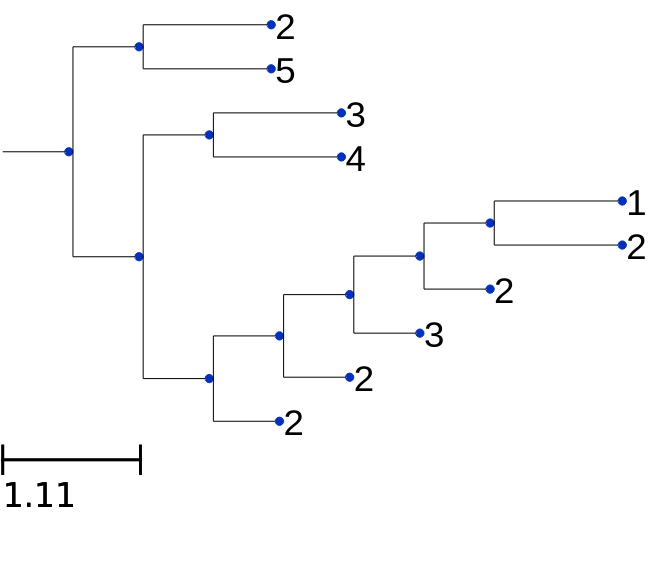
\includegraphics[scale=0.6]{tier1.png}
\caption{GB-UNSAT tree in original polynomial order}
\label{fig:tier1}
\end{figure}

In this graph, longer edges (1 unit length) denote s-poly pairs and shorter edges (0.5 unit length) denote
polynomials used for division/reduction. Illustration of this graph: s-poly of $(1,2)$ could be divided by $f_2,f_3$
and s-poly generated by $(3,4)$ and $(2,5)$. UNSAT core attained using this GB computation method is $\{1,2,3,4,5\}$.
However, the minimal core is $\{1,2,4,5\}$ so $f_3$ is "redundant" here, but it is not 
on the longest path.
\end{Example}

This example violates conjecture \ref{conj:original}. Still, we notice the "redundant" $f_3$ could be found in other
minimal cores. In fact, there are at least 4 minimal cores for this set of polynomials:
\begin{align*}
& \{1,2,3,4,7,8\}
& \{2,4,5,6,8\}
& \{2,3,4,6,8\}
& \{1,2,4,5\}
\end{align*}

Maybe we can refine our conjecture like this:
\begin{Conjecture}
\label{conj:refine}
Any polynomial which is included by GB computation method but not in any minimal core will be on the longest path.
\end{Conjecture}

To verify this conjecture we will need to perform more non-trivial but reasonably-small experiments.

\section{Smaller UNSAT core extraction}
If an analytical method for minimal UNSAT core extraction is intractable, we may want to get UNSAT core as small as possible.
To achieve this goal with limited number of iterations, we may need following conjecture:
\begin{Conjecture}
By carefully arranging the order of picking s-poly pairs, we can always get a new core whose size is no larger than
last iteration.
\end{Conjecture}

Or we can loose the constrain:
\begin{Conjecture}
By carefully arranging the order of picking s-poly pairs, the probability that we get a smaller core
is much higher than the probability that we get a larger core.
\end{Conjecture}

Here I will propose a simple rearrange strategy, which works at least for Ex.\ref{exi}:

\emph{After getting an UNSAT core, we can rearrange the order of polynomials by following criteria:\\
i. Polynomials in the core come first;\\
ii. Polynomial with a shorter distance to refutation "1" comes first;\\
iii. When there are 2 polynomials with the same distance, the one appears more frequently in the tree comes first.}

\begin{Example}
Let us make Ex.\ref{exi} as the first iteration, we get a core $\{1,2,3,4,5\}$. Check out Fig.\ref{fig:tier1},
we can rearrange polynomials as
$$\{2,5,4,3,1,6,7,8,9\}$$
Run our approach using this order, we get a new core $\{1,2,4,5\}$, as Fig.\ref{fig:tier2} shows:
\begin{figure}[hbt]
\centering
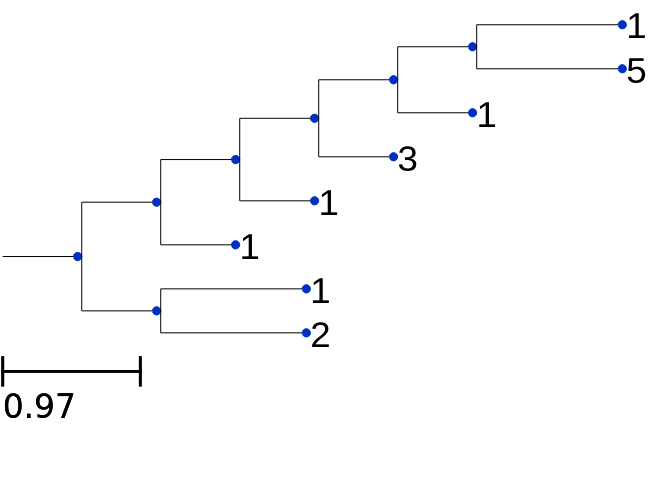
\includegraphics[scale=0.6]{tier2.png}
\caption{GB-UNSAT tree after rearranging polynomial order}
\label{fig:tier2}
\end{figure}
Note "1 2 3 5" here are new indices corresponding to original $f_1,f_2,f_4,f_5$. Applying the criteria
we further rearrange polynomials as
$$\{2,5,4,1,3,6,7,8,9\}$$
Run our approach again, the result is still core $\{1,2,4,5\}$, which is minimal. Notice we arrive a fixpoint.
\end{Example}

Again, my conjecture need more experiments. I will keep updating and discussions are welcome.